\documentclass[11pt,a4paper]{report}
\usepackage[utf8]{inputenc}
\usepackage[T1]{fontenc}
\usepackage{lmodern}
\usepackage{microtype}
\usepackage[a4paper,margin=2.5cm]{geometry}
\usepackage{amsmath,amssymb,amsfonts,bm}
\newcommand{\R}{\mathbb{R}}
\usepackage[numbers,sort&compress]{natbib}
\usepackage{booktabs}
\usepackage{graphicx}
\usepackage{tikz}
\usetikzlibrary{arrows.meta,positioning}
\usepackage{caption}
\usepackage{subcaption}
\usepackage[hidelinks,linktoc=all]{hyperref}
\usepackage{bookmark}

% Canonical path first; debiased folder is a secondary override/source.
\graphicspath{{outputs/figures/}{debiased_outputs/figures/}}

\title{Measuring Popularity Bias, Fairness for Users, and Feedback Loops in Recommender Systems}
\author{Cebo Mkhwanazi}
\date{March 2026}

\begin{document}
\hypersetup{
  pdftitle={Measuring Popularity Bias, Fairness for Users, and Feedback Loops in Recommender Systems},
  pdfauthor={Cebo Mkhwanazi}
}

\maketitle

\chapter*{Declaration}
\addcontentsline{toc}{chapter}{Declaration}
Standard Stellenbosch University declaration of original work.

\chapter*{Abstract}
\addcontentsline{toc}{chapter}{Abstract}
Recommender Systems (RS) are critical tools for content discovery, yet many algorithms fail to promote diverse content, instead exhibiting a measurable popularity bias—the disproportionate recommendation of already popular items. This phenomenon leads to significant exposure disparity, reinforcing market imbalances and restricting user access to niche content. This thesis presents a rigorous empirical study that detects and quantifies inherent popularity and exposure bias across classical Collaborative Filtering (CF) architectures and Content-Based models. 

Using standard benchmark datasets (MovieLens, Last.fm, Book-Crossing) alongside a proprietary, highly sparse e-commerce dataset from Takealot, the study implements a unified, three-phase evaluation framework. \textbf{Experiment A} measures macro-level exposure bias, revealing that Matrix Factorization models (SVD, ALS) act as extreme popularity amplifiers, exhibiting near-perfect Gini coefficients and collapsing catalog coverage on sparse data. \textbf{Experiment B} investigates user-centric fairness, quantifying a "niche tax" where models significantly degrade in ranking quality (NDCG@10) and predictive accuracy (RMSE) for users with non-mainstream tastes. \textbf{Experiment C} employs a longitudinal feedback simulation to demonstrate how CF models drive diversity decay over time, while content-based models show resilience against filter bubbles.

The results provide quantitative evidence that architectural differences significantly contribute to bias amplification, independent of the underlying data distribution. The severe exacerbation of these biases in the sparse Takealot environment highlights the danger of relying solely on dense academic benchmarks for model selection. These findings underscore the necessity of adopting holistic evaluation metrics beyond traditional accuracy, and demonstrate that mitigating algorithmic concentration is essential to ensure long-term ecosystem health and fairness in digital platforms.

\chapter*{Acknowledgements}
\addcontentsline{toc}{chapter}{Acknowledgements}
Thanking supervisors, funding bodies, and Takealot.

\tableofcontents
\newpage
\listoffigures
\listoftables

\chapter*{List of Abbreviations}
\addcontentsline{toc}{chapter}{List of Abbreviations}
Crucial addition for CS/Data Science: Define NDCG, RMSE, SVD, ALS, TF-IDF, ARP, etc., here so you don't clutter the main text.

\newpage

\chapter{Introduction}
\label{ch:introduction}
% Sets the stage, formally states the problem, and outlines exactly what this thesis contributes.

\section{Context and Motivation}
% The explosive growth of recommender systems in digital platforms.
Personalized recommender systems are the primary mechanisms through which users discover new content on modern digital platforms, from streaming services to large-scale e-commerce marketplaces. These systems operate by learning from historical user interactions. Because historical engagement naturally exhibits a skew where a small fraction of items receives the majority of attention, recommendation algorithms tend to learn and amplify this pattern. This phenomenon, known as popularity bias, causes systems to disproportionately recommend blockbuster items while systematically under-representing the "long tail" of the catalog.

\subsection{Technical, Social, and Economic Imperatives}
Addressing this bias is not merely a theoretical computer science problem; it is driven by critical technical, social, and economic imperatives. 

From a \textbf{technical perspective}, optimizing purely for historical "accuracy" (e.g., minimizing error on past clicks) is fundamentally flawed. When algorithms act as popularity amplifiers, they fail at their primary goal of \textit{discovery}. A system that only recommends items a user would have easily found anyway provides little technical utility and suffers from catalog starvation, exposing only a fraction of the available inventory.

From a \textbf{social perspective}, unchecked algorithmic bias creates profound real-world consequences, most notably the creation of "filter bubbles." When recommendation engines consistently narrow the scope of content shown to users, they limit diverse viewpoints, homogenize user experiences, and systematically disadvantage users who have unique or niche preferences. The social imperative demands systems that are fair not just to the mainstream majority, but to all consumer segments.

Finally, the \textbf{economic imperative} is perhaps the most urgent for digital marketplaces. Platforms like Takealot rely on a vast ecosystem of third-party vendors. When popularity bias dictates visibility, it creates a "winner-takes-all" economy \citep{anderson2004long}. Niche vendors and emerging products are algorithmically suppressed, driving them out of the marketplace. For the platform, this reduces long-term resilience, as a healthy e-commerce ecosystem requires a thriving long tail, not just a dominant top tier.

\section{Problem Statement}
While the existence of popularity and exposure bias is documented, significant gaps remain regarding their comparative manifestation across different algorithmic families and dataset sparsity levels. The core problem explored in this research is the lack of a standardized baseline to characterize how specific architectures amplify these biases, particularly when transitioning from dense academic datasets to sparse, real-world e-commerce environments. This study addresses the following critical gaps:

\begin{enumerate}
    \item \textbf{The Matthew Effect in algorithmic cycles:} Popularity bias creates self-reinforcing cycles where mainstream dominance is reinforced at the expense of content diversity.
    \item \textbf{Incomplete characterization across algorithms:} There is a lack of comparative analysis examining how bias propagation differs between memory-based methods ($k$-NN), model-based systems (SVD/ALS), and content-based approaches (TF-IDF, Logistic Regression).
    \item \textbf{Insufficient user-centric analysis:} System-level statistics often overlook how different user segments (e.g., niche-focused vs. mainstream-focused) are differentially impacted, leading to an unfair "niche tax."
    \item \textbf{Quality-bias trade-offs:} The relationship between ranking quality (e.g., NDCG) and fairness remains poorly understood in unmitigated environments.
\end{enumerate}

\section{Research Objectives and Questions}
% * RQ1: How concentrated are recommendations across items under different algorithmic paradigms? (Maps to Chapter 4)
% RQ2: How do accuracy and ranking metrics disparate across varying user segments, specifically mainstream vs. niche users? (Maps to Chapter 5)
% RQ3: Under a stylized longitudinal feedback process, how do diversity and popularity-related metrics evolve? (Maps to Chapter 6)
This study breaks them down into three main questions about what items get shown, how fair the system is to individuals, and what happens over time:

\begin{itemize}
    \item \textbf{RQ1:} How concentrated are recommendations across items under different algorithmic paradigms?
    \item \textbf{RQ2:} How do accuracy and ranking metrics disparate across varying user segments, specifically mainstream vs. niche users?
    \item \textbf{RQ3:} Under a stylized longitudinal feedback process, how do diversity and popularity-related metrics evolve?
\end{itemize}

\section{Scope and Limitations}

\subsection{Focus Area}
This research is scoped to focus specifically on popularity bias and exposure bias in the context of both explicit and implicit feedback recommender systems. The study explores how these biases manifest at the macro-level (catalog coverage), micro-level (user fairness), and longitudinally over time. It specifically investigates whether architectural design choices—rather than just the data—drive bias amplification.

The research does \textbf{not} cover demographic or representation bias (e.g., based on gender or ethnicity), nor does it evaluate online A/B testing in live production environments, as all evaluations are conducted offline using historical datasets and simulations.

\subsection{System Scale and Constraints}
To ensure methodological rigor while maintaining feasibility, this study focuses on:
\begin{itemize}
    \item \textbf{Algorithms:} Well-established baseline, neighborhood, matrix factorization, and content-based algorithms. Deep learning approaches (e.g., NeuMF) requiring extensive computational resources are excluded to allow for controlled, isolated testing of foundational bias mechanisms.
    \item \textbf{Datasets:} A mix of publicly available dense benchmarks (MovieLens, Last.fm, Book-Crossing) and a proprietary, ultra-sparse e-commerce dataset (Takealot), limiting generalizability strictly to these specific sparsity profiles.
\end{itemize}

\subsection{Methodological Limitations}
Offline metrics are imperfect proxies for online performance and may not fully capture real-world user satisfaction. Furthermore, the longitudinal feedback loop simulation (Experiment C) relies on a stochastic user choice model; while grounded in theoretical probabilities, it cannot perfectly capture dynamic human responses. Finally, the evaluation of content-based models via RMSE introduces methodological artifacts due to the necessity of mean-fallback placeholders for unpredicted items.

\section{Key Contributions}
% Highlight the unified evaluation protocol, the contrast between public dense datasets and the sparse proprietary Takealot dataset, and the testing of debiasing interventions.
Most research on recommender systems only looks at very dense and clean datasets, like the MovieLens movie ratings. These datasets do not look like real, messy, and very large online stores. The main new idea in this research is comparing different types of data. This thesis directly compares four standard public datasets with a huge, very sparse e-commerce dataset from the Takealot store. By comparing these, this research finds that matrix factorization models fail completely in sparse datasets, mostly showing nothing but the top few items. It also proves that content-based models naturally avoid getting trapped in filter bubbles over time.

\section{Thesis Outline}
% A brief roadmap of the remaining chapters.

\chapter{Literature Review}
\label{ch:lit_review}
% Contextualizes your work within the broader academic discourse and identifies the gaps your thesis fills.

\section{Recommender Systems Paradigms}
Recommender systems have evolved from early rule-based filtering to sophisticated machine learning architectures that power content discovery across e-commerce, streaming media, social platforms, and news aggregation.

\subsection{Filtering Paradigms and Algorithmic Families}
\textbf{Collaborative Filtering (CF)} operates on the principle that users who agreed in the past will agree in the future \citep{sarwar2001item}. It can be \textbf{memory-based} (neighborhood methods such as User-KNN and Item-KNN) or \textbf{model-based} (latent factor models such as SVD and matrix factorization) \citep{koren2009matrix}. CF requires no item metadata and benefits from the collective behavior of many users, but it suffers from the cold-start problem for new users or items and is vulnerable to data sparsity.

\textbf{Content-Based Filtering} recommends items similar to those a user has previously liked, using item attributes (e.g., genre, director, tags). It does not rely on other users' behavior and can recommend new items immediately. However, it tends to produce narrow, homogeneous recommendations and struggles with the ``filter bubble'' effect.

\textbf{Hybrid approaches} combine CF and content-based methods to leverage the strengths of both, often achieving better accuracy and coverage than either approach alone.

\subsection{Explicit vs. Implicit Feedback}
A critical distinction in recommendation data is between \textbf{explicit feedback} (e.g., star ratings, likes) and \textbf{implicit feedback} (clicks, views, purchases) \citep{hu2008collaborative}. Explicit feedback directly expresses preference strength but is sparse and subject to selection bias. Implicit feedback is abundant and reflects actual behavior but is ambiguous: the absence of an interaction does not necessarily indicate disinterest---it may indicate lack of exposure.

\subsection{Modern Approaches (Deep Learning \& Graphs)}
% A brief look at architectures like Neural Collaborative Filtering (NeuMF) and Graph Convolutional Networks (LightGCN), justifying why foundational baselines are better suited for isolated bias testing.

\section{Theoretical Foundations of Bias}
% Grounding the exposure problem formally.

\subsection{Rubin's Missing Data Framework}
% Discussing Missing Completely at Random (MCAR) vs. Missing Not at Random (MNAR) in recommendation logs.

\subsection{Inverse Propensity Score (IPS) Methods}
% The mathematical gold standard for adjusting exposure bias.

\section{Popularity and Exposure Bias: The Bias Propagation Chain}
% A conceptual model of how bias spreads from historical data, to model training, to user exposure.
Popularity and exposure biases are some of the biggest problems in modern recommendation systems. Traditional collaborative filtering looks for matches based on what items are bought together. This means standard collaborative algorithms try to be accurate by just guessing the most famous items.

Current research measures this unequal exposure using common economic methods. Gini coefficients are widely used to see how crowded the system's recommendations are. This shows clearly that algorithms act like loud speakers for popular items. The research strongly agrees that standard machine learning methods punish the system for exploring rare items. This forces developers to use extra tricks to fix the rankings after the model runs.

\section{User-Centric Fairness \& Disparate Impact}
Fairness in recommender systems is now split into two main areas. Provider fairness is about giving all sellers or artists a fair chance. Consumer fairness is about giving good recommendations to all types of users.

\subsection{The Accuracy-Fairness Tension}
Historically, recommender systems have been optimized primarily for \textbf{accuracy metrics} such as Root Mean Squared Error (RMSE) and Normalized Discounted Cumulative Gain (NDCG). However, observed data is biased: it reflects exposure patterns and historical inequities. Optimizing for accuracy on biased data can amplify these biases, creating a tension between accuracy and fairness. As \citet{ekstrand2022fairness} and \citet{abdollahpouri2019managing} argue, systems that maximize accuracy may simultaneously maximize popularity bias and reduce diversity.

Within consumer fairness, recent studies have found a problem called the "niche tax." Because users with unique tastes share fewer items with the rest of the group, algorithms have a hard time finding similar users to compare them to. This problem directly leads to higher error rates for users who like rare items, compared to users who like popular items. \citet{abdollahpouri2020multistakeholder} demonstrated this relationship, revealing that user groups are affected differently by algorithmic popularity bias depending on their inherent interest in popular items. They introduced the $\Delta$GAP metric to quantify disparities between mainstream-focused and niche-focused user groups.

\section{Temporal Dynamics \& Feedback Loops}
% How logged data and closed-world recommendations interact to create filter bubbles.
The idea of the filter bubble was first used to describe how people get trapped seeing only news they agree with \citep{chaney2018algorithmic}. In online shopping and media, it means the system forces users to see a narrower range of items over time. As users click mostly on the items the computer shows them, the system learns only from its own past choices. This leads to everything looking the same, a process called diversity decay \citep{mansoury2020feedback}.

Running computer simulations over multiple steps is needed to really understand how recommendations work as active, changing loops instead of just simple, fixed guessing tasks.

\section{Mitigation Strategies: A Methodological Survey}
% Reviewing pre-processing, in-processing, and post-processing interventions.

\section{The Research Gap}
% The need for comparable metrics across disparate models and domains (entertainment vs. e-commerce).

\chapter{Methodology and Experimental Framework}
\label{ch:methodology}
% The comprehensive blueprint. This merges your datasets, algorithms, and academic rigor into one cohesive foundation.

\section{Research Design Overview}
% Introduction to the three-phase pipeline (Experiment A, B, and C).
To fully study these three bias problems in recommender systems, this study uses a clear, numbers-based plan across different types of data. The testing setup compares six types of algorithms on five different datasets. This covers both crowded movie-rating data and very sparse online shopping data.

The testing plan is split into three steps:
\begin{enumerate}
    \item \textbf{Experiment A (Macro-Level Exposure Bias):} Checking how the system recommends items overall and how much of the store actually gets shown.
    \item \textbf{Experiment B (User-Centric Fairness):} Grouping users by their past choices to see if the system works worse for some groups.
    \item \textbf{Experiment C (Longitudinal Feedback Dynamics):} Running a loop that guesses user clicks over multiple steps to see what happens in the long run.
\end{enumerate}

\begin{figure}[htbp]
  \centering
  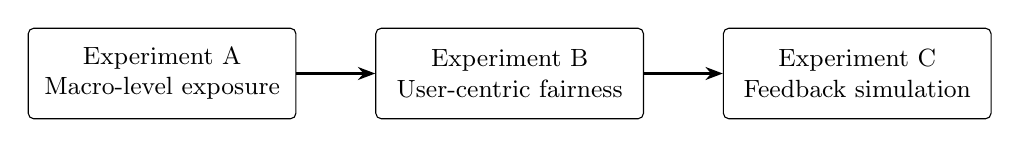
\begin{tikzpicture}[
      node distance=0.6cm and 1.0cm,
      box/.style={rectangle, draw, rounded corners=2pt, minimum width=3.4cm, minimum height=1.15cm, align=center, font=\small},
      arr/.style={-{Stealth[length=2.2mm]}, thick},
    ]
    \node[box] (a) {Experiment A\\Macro-level exposure};
    \node[box, right=of a] (b) {Experiment B\\User-centric fairness};
    \node[box, right=of b] (c) {Experiment C\\Feedback simulation};
    \draw[arr] (a) -- (b);
    \draw[arr] (b) -- (c);
  \end{tikzpicture}
  \caption{The three main steps of the testing plan.}
  \label{fig:pipeline}
\end{figure}

\section{Datasets and Domains}
% Detail MovieLens (100K/1M), Last.fm 2K, Book-Crossing, and explicitly contrast them with the schema and sparsity of the proprietary Takealot dataset.
Standard academic datasets do not show the real problems of large, empty online stores. Because of this, the study tests models on data with different levels of crowding.

\textbf{Public Datasets:}
\begin{itemize}
    \item \textbf{MovieLens 100K and 1M} \citep{harper2015movielens}: Crowded, clear movie datasets. The item details are simple words for movie genres.
    \item \textbf{Last.fm 2K} \citep{cantador2011second}: A dataset showing how many times a song was played. The play numbers were grouped into clear ratings from 1 to 5. Item details are made by combining artist names and user tags.
    \item \textbf{Book-Crossing} \citep{ziegler2005improving}: A sparse dataset of book ratings. Empty links with no real ratings were removed to keep the error testing exact.
\end{itemize}

\textbf{E-Commerce Data (Takealot Dataset):}
To anchor the study in the real world, a large, private data snapshot from the Takealot online store was used. This dataset is special because it has a massive number of rare items and is very sparse. The inputs were taken from customer reviews, and the item details were made by linking product names, brand names, and store categories together.

\section{Data Preprocessing}
Let $G_0$ be the interaction bipartite graph. For chosen thresholds $(k_U,k_I)$ (both $10$ in code), the $k$-core filtering strategy repeats the following until convergence:
\begin{equation}
  \mathcal{U}_{t+1} = \bigl\{ u : \deg_{G_t}(u) \ge k_U \bigr\}, \qquad
  \mathcal{I}_{t+1} = \bigl\{ i : \deg_{G_t}(i) \ge k_I \bigr\},
\end{equation}
keeping only edges between $\mathcal{U}_{t+1}$ and $\mathcal{I}_{t+1}$, then sets $G_{t+1}$ accordingly. This removes tail users and items, yielding a denser core for more stable collaborative estimates.

\section{Ethics and Data Use}
% Acknowledgement of public benchmark licenses and the specific usage constraints and anonymization of the Takealot data.

\section{Algorithmic Baselines \& Constraints}
The setup tests six recommendation models across collaborative and content-based paradigms:

\begin{itemize}
    \item \textbf{User-Based $k$-NN (Surprise):} Uses cosine similarity and user-based aggregation to provide predictions $\hat{r}_{ui}$.
    \item \textbf{SVD (Biased Probabilistic Matrix Factorization):} Uses \texttt{surprise.SVD}, optimizing regularized squared error on observed ratings with latent factors and bias terms.
    \item \textbf{ALS (Implicit Library):} Fits alternating least squares on a sparse user$\times$item matrix with nonzeros $r_{ui}$ from training ratings (factors$=50$, iterations$=15$, regularization$=0.01$).
    \item \textbf{TF--IDF Profile Model:} Represents items with TF-IDF vectors $\bm{v}_i \in \R^d$ of metadata. A user $u$'s profile is $\bar{\bm{v}}_u = \frac{1}{|H_u|} \sum_{i \in H_u} \bm{v}_i$, and items are scored via cosine similarity.
    \item \textbf{Per-User Logistic Regression:} Defines a binary label $y=1$ if $r_{ui}$ is at or above the user's median rating. A pipeline of TF-IDF and logistic regression predicts $\mathbb{P}(y=1|\text{metadata})$ for candidates.
    \item \textbf{Random Forest on IDs:} User and item identifiers are label-encoded, and a random forest regressor predicts $\hat{r}_{ui}$ from the pair $(u,i)$ only, capturing memorized popularity structure without text.
\end{itemize}

\section{Evaluation Metrics Formulations}

\subsection{Macro-Level Metrics (Distributional Equity)}

\subsubsection*{1. Gini Index}
The Gini Index assesses recommendation distribution inequality, showing perfect equality at 0 and maximal inequality at 1 \citep{cowell2011measuring}.
\begin{equation}
G = \frac{\sum_{i=1}^{n}\sum_{j=1}^{n}|x_i - x_j|}{2n^2\bar{x}}
\end{equation}
where $x_i$ represents the recommendation frequency of item $i$, $n$ is the total number of items, and $\bar{x}$ is the mean recommendation frequency.

\subsubsection*{2. Catalogue Coverage}
This metric quantifies the percentage of unique items recommended to users.
\begin{equation}
\textrm{Coverage} = \frac{|\{i \in I : \textrm{item } i \textrm{ is recommended}\}|}{|I|} \times 100\%
\end{equation}
where $I$ represents the full item catalogue.

\subsubsection*{3. Group Average Popularity (GAP) and $\Delta$GAP}
GAP measures the average popularity of items recommended to a user group $g$. $\Delta$GAP quantifies disparities between groups (e.g., mainstream vs. niche-focused users).
\begin{align}
\textrm{GAP}_g &= \frac{1}{|U_g|}\sum_{u \in U_g}\frac{1}{|R_u|}\sum_{i \in R_u}\textrm{pop}(i) \\
\Delta\textrm{GAP} &= |\textrm{GAP}_{g1} - \textrm{GAP}_{g2}|
\end{align}
where $\textrm{pop}(i)$ is an item's interaction count, $U_g$ is a user group, and $R_u$ is user $u$'s recommendations.

\subsubsection*{4. Exposure Fairness}
Evaluates how equitably items are visible in recommendations using entropy $H(E)$.
\begin{equation}
H(E) = -\sum_{i=1}^{n}p_i\log p_i \quad \textrm{where} \quad p_i = \frac{\textrm{Exposure}(i)}{\sum_{j=1}^{n}\textrm{Exposure}(j)}
\end{equation}

\subsubsection*{5. Average Recommendation Popularity (ARP)}
Measures the average popularity of recommended items:
\begin{equation}
\textrm{ARP} = \frac{1}{|U|}\sum_{u \in U} \frac{1}{|R_u|}\sum_{i \in R_u} \textrm{pop}(i)
\end{equation}

\subsection{Micro-Level Metrics (Ranking Quality \& Accuracy)}
While macro metrics capture fairness, standard micro-level metrics including \textbf{NDCG@10} and \textbf{RMSE} are utilized to ensure that fairness interventions are evaluated against the traditional predictive baseline, observing the quality-bias trade-off curve.

\section{Statistical Testing Framework}
% Detailing the tests used (e.g., Mann-Whitney, Welch) to ensure observed differences are statistically significant.

\section{Implementation and Reproducibility}
Core numerical tooling uses NumPy and Pandas; scikit-learn supplies TF-IDF, logistic regression, random forests, and cosine similarity. Surprise provides $k$-NN and SVD (with a bias-only fallback if unavailable). ALS uses the \texttt{implicit} library. Reproducibility is guaranteed via isolated pipelines (e.g., \texttt{run\_all.py} and \texttt{run\_takealot\_full.py}). 

\textbf{Known Limitations:}
\begin{itemize}
    \item \textbf{Segment RMSE for ALS, TF--IDF, LogReg:} The implementation assigns the global training mean prediction to every test row for RMSE computation for these models, while still computing genuine top-$K$ lists for NDCG. Therefore niche, diverse, and mainstream RMSE are \emph{identical} within each of these model families on a given dataset. Only k-NN, SVD, and Random Forest provide differentiated segment RMSE.
    \item \textbf{ALS robustness:} Failures fall back to trivial recommendations (first catalog items), which can artifactually inflate concentration metrics.
\end{itemize}

\chapter{Experiment A - Macro-Level Exposure Bias}
\label{ch:exp_a}
% Anchor Visual: Heatmaps from combined_figures.py showing item exposure concentration.

\section{Experimental Setup}
% Parameters for top-K list generation across datasets.
Models generated top 10 lists for all test users to see how the items were spread out:
\begin{itemize}
    \item \textbf{Gini Inequality Check}: Measured how unbalanced the total recommendations were.
    \item \textbf{Catalog Coverage Check}: Counted what percentage of the whole store was ever actually shown to anyone.
    \item \textbf{Average Recommendation Popularity (ARP)}: Checked how popular the suggested items already were in the past.
\end{itemize}

\section{Algorithmic Amplification in Collaborative Models}
The results demonstrate a stark contrast in how different algorithmic families distribute exposure. Matrix factorization models proved highly susceptible to popularity bias. 

\begin{figure}[htbp]
  \centering
  \begin{subfigure}[t]{0.48\textwidth}
    \centering
    
\includegraphics[width=\linewidth]{combined_macro_gini_heatmap.png}
    \caption{Gini coefficient on recommendation frequency (model $\times$ dataset).}
    \label{fig:macro-gini}
  \end{subfigure}\hfill
  \begin{subfigure}[t]{0.48\textwidth}
    \centering
    
\includegraphics[width=\linewidth]{combined_macro_catalog_coverage_heatmap.png}
    \caption{Catalog coverage of recommended items (model $\times$ dataset).}
    \label{fig:macro-cov}
  \end{subfigure}
  \caption{Macro-level exposure inequality and coverage across benchmarks (including Takealot). Darker cells in the Gini heatmap indicate stronger concentration on a few items.}
  \label{fig:macro-heatmaps}
\end{figure}

Across datasets, ALS averaged a Gini coefficient of $\sim 0.99$, indicating severe inequality. As seen in Figure \ref{fig:macro-cov}, on the massive Takealot catalog, ALS achieved a catastrophic catalog coverage of 0.00029\%, recommending only 14 unique items to the entire user base. SVD similarly demonstrated strong positive Spearman correlations (e.g., 0.43 on ML-100K) between training popularity and recommendation frequency.

\section{Exposure Dispersal via Content Models}
Content models successfully distributed exposure into the long tail. Logistic Regression achieved the highest catalog coverage across the board (e.g., 93\% on ML-1M, 56.3\% on Takealot), effectively acting as a discovery engine decoupled from global interaction frequency.

\begin{table}[htbp]
  \centering
  \caption{Representative macro-bias values: ALS vs.\ Logistic Regression.}
  \label{tab:macro-numbers}
  \begin{tabular}{@{}llrr@{}}
    \toprule
    \textbf{Dataset} & \textbf{Model} & \textbf{Gini} & \textbf{Catalog cov.} \\
    \midrule
    Takealot & ALS & 0.9998 & 0.00029 \\
    Takealot & LogReg & 0.733 & 0.563 \\
    MovieLens 100K & ALS & 0.987 & 0.033 \\
    MovieLens 100K & LogReg & 0.543 & 0.887 \\
    \bottomrule
  \end{tabular}
\end{table}

\section{Domain Contrast Results}
% The severe exacerbation of biases when moving from dense public datasets to the ultra-sparse Takealot environment.

\section{Intervention (Post-Processing)}
% Testing a debiasing intervention (applying a popularity penalty) on collaborative models.
A special extra rule, called SVD+Rerank, is used to punish items just for being popular. By changing both the guessed score and the overall popularity count to a simple range, it lowers the score of very popular items based on a fixed setting.

\section{Summary of Findings}
% Directly answering RQ1.

\chapter{Experiment B - User-Centric Fairness (The "Niche Tax")}
\label{ch:exp_b}
% Anchor Visual: The combined_rmse_niche_vs_mainstream.png chart.

\section{User Stratification Strategy}
For each user $u$, we define the \emph{mainstreaminess} score:
\begin{equation}
  M_u = \frac{1}{|H_u|} \sum_{i \in H_u} p_i ,
\end{equation}
where $H_u$ is user $u$'s training item set and $p_i$ is the item's global training interaction count. Users are split into tertiles based on this score: \textbf{Niche} (low $M_u$), \textbf{Diverse} (middle), and \textbf{Mainstream} (high).

\section{The RMSE Methodological Artifact}
% A deep dive into why evaluating content models via RMSE on sparse segments introduces systemic flaws due to mean-fallback placeholders.
An important point in this test is that text-based models do not naturally guess exact rating numbers. When checking the error (RMSE) for user groups on these models, the system had to just guess the average score to make it work. Because of this, comparing RMSE mostly shows the flaws in collaborative models.

\section{Predictive Disparities}
Analysis of the $\Delta$ Accuracy metric ($\mathrm{RMSE}_{\text{niche}} - \mathrm{RMSE}_{\text{mainstream}}$) revealed that users with unique tastes frequently receive substandard algorithmic service.

\begin{figure}[htbp]
  \centering
  
\includegraphics[width=0.92\textwidth]{combined_fairness_gap_delta_rmse.png}
  \caption{Fairness gap $\Delta\mathrm{RMSE} = \mathrm{RMSE}_{\text{niche}} - \mathrm{RMSE}_{\text{mainstream}}$ by dataset and model. Positive values indicate higher error for niche users. Note that content models that fall back to a global mean for rating prediction can show flat $\Delta\mathrm{RMSE}$; segment NDCG should be read alongside this chart.}
  \label{fig:fairness-gap}
\end{figure}

\begin{figure}[htbp]
  \centering
  
\includegraphics[width=0.92\textwidth]{combined_rmse_niche_vs_mainstream.png}
  \caption{RMSE by user segment (Niche vs.\ Mainstream) across datasets and models.}
  \label{fig:rmse-segment}
\end{figure}

\textbf{Neighborhood Penalties:} As shown in Figures \ref{fig:fairness-gap} and \ref{fig:rmse-segment}, k-NN models consistently exhibited a positive ``niche tax,'' peaking on the Book-Crossing dataset with a gap of 0.1127. This confirms that finding reliable behavioral peers for niche users in sparse data is highly challenging.

\textbf{The Latent Space Anomaly:} Interestingly, SVD on Last.fm 2K produced a negative gap ($-0.1140$), indicating that matrix factorization can occasionally model niche clusters more accurately than mainstream noise.

\section{Ranking Fairness (NDCG@10)}
Evaluating the ``niche tax'' revealed the critical limitations of standard error metrics. Because content models optimize for ranking rather than explicit rating prediction, shifting the analysis to NDCG@10 exposes the true ranking disparity. On dense datasets like MovieLens 100K, content models provided significantly more equitable NDCG scores across niche and mainstream segments compared to k-NN, which heavily penalized niche users. Conversely, in the massive Takealot catalog, NDCG@10 was universally low ($< 0.02$) across all segments, indicating that the sheer scale of the item space overshadows algorithmic attempts at fair ranking.

\section{Summary of Findings}
% Directly answering RQ2.

\chapter{Experiment C - Longitudinal Feedback Dynamics}
\label{ch:exp_c}
% Anchor Visual: The combined_feedback_diversity_decay.png lines chart showing iteration over iteration.

\section{Simulation Design}
The simulation initializes a training log $\mathcal{D}_0$ as an 80\% random sample of all ratings. For rounds $t=1,\ldots,5$ and for each model in $\{\text{SVD}, \text{TF--IDF}\}$:
\begin{enumerate}
  \item Train on $\mathcal{D}_{t-1}$, recommend top-$5$ unseen items per user.
  \item Compute relevance score $s_{ui}$ from model outputs (normalized predicted rating for SVD; cosine score for TF--IDF).
  \item Let $\tilde{p}_i$ be training popularity in $\mathcal{D}_{t-1}$, min--max normalized to $[0,1]$. Simulate clicks.
  \item Append clicked pairs as ratings $5.0$; resolve duplicates on $(u,i)$ keeping the last event, yielding $\mathcal{D}_t$.
\end{enumerate}

\section{The Stochastic User Choice Model}
% Mathematical formulation bridging relevance and popularity to simulate clicks.
The click logic used a simple mix to balance how accurate the guess was versus how famous the item already was:
\begin{equation}
    P(click_{u,i}) = \max\bigl(0,\, \min\bigl(1,\, 0.7 \cdot \text{Rel}(u,i) + 0.3 \cdot \text{Pop}_{norm}(i)\bigr)\bigr)
\end{equation}
Using the 0.7 mix makes sure the fake clicks act like real platform users, combining user interest with crowd hype.

\section{Collaborative "Popularity Creep"}
The 5-iteration simulation challenged the monolithic concept of ``diversity decay''.

\begin{figure}[htbp]
  \centering
  
\includegraphics[width=0.92\textwidth]{combined_feedback_diversity_decay.png}
  \caption{Feedback simulation: aggregate diversity (unique recommended items) and ARP over five iterations for SVD and TF-IDF, by dataset. Trajectories illustrate how collaborative vs.\ content-based models respond to synthetic clicks.}
  \label{fig:feedback-diversity}
\end{figure}

SVD consistently amplified historical biases over time. In ML-1M, SVD's ARP grew from 893 to 1997, actively shrinking its aggregate diversity.

\section{Content Model Resilience}
TF-IDF demonstrated an ability to resist the filter bubble effect. In ML-100K and ML-1M, TF-IDF actually increased its aggregate diversity over sequential iterations. This indicates that leveraging item attributes can break the recursive feedback loop caused by pure collaborative filtering.

\section{Summary of Findings}
% Directly answering RQ3.

\chapter{Discussion}
\label{ch:discussion}
% Synthesizing the three experiments and demonstrating critical academic thought.

\section{The Interconnectedness of Biases}
% Synthesizing how macro-level catalog starvation (Ch 4) drives the micro-level niche tax (Ch 5) and is compounded by feedback loops (Ch 6).

\section{The Domain Extreme}
% Reiterating that algorithmic choices that work for standard dense benchmarks fail gracefully on sparse e-commerce data like Takealot.
Only testing on normal, crowded academic data gives researchers a false sense of how good a model is. Moving to test on real, sparse data, like the Takealot dataset, proves a major point. It shows that using plain collaborative matrix models in real online stores causes a total failure in showing users a healthy mix of items.

\section{Threats to Validity}
% A critical self-assessment. Acknowledging simulation assumptions, the limitation of penalizing popularity, and segment definitions.
A major limit in this setup was the problem of comparing basic numeric errors on simple number rating scales. Text models that use shapes and distances to guess items had to use basic average numbers to fill in the blanks. This limited how exact the fairness error gap could be measured on these models without ruining the standard sorting ranks. Future work should build custom testing layers that handle these error matches much better.

\section{Implications for Practitioners}
% Real-world consequences for marketplace health and vendor equitability.
For companies running real stores, the findings suggest moving away from using only matrix math models. By slowly adding in text models like TF-IDF or setting custom fixed limits, developers can stop filter bubbles from building up smoothly. Knowing what the algorithms do badly allows companies to make sure many different items are found, while still making useful sales suggestions.

\chapter{Conclusion}
\label{ch:conclusion_final}

\section{Summary of the Study}
This thesis empirically demonstrates that popularity bias is heavily model-dependent and domain-sensitive. By stepping outside traditional, dense movie benchmarks and utilizing the Takealot e-commerce corpus, this study revealed that standard matrix factorization models (ALS) collapse into extreme exposure inequality (Gini $\sim 0.9998$) when faced with massive, sparse catalogs. Furthermore, longitudinal simulations utilizing a formal stochastic user choice model proved that collaborative filtering actively amplifies this bias over time, whereas content-based architectures demonstrate resilience, preserving or expanding aggregate diversity.

Finally, this study highlights a critical gap in industry evaluation protocols: the inability to directly compare the user-centric predictive accuracy (RMSE) of latent-factor models against content-based models without resorting to global mean fallbacks. Recommender systems must be audited not just for aggregate accuracy, but for how equitably they distribute exposure and accuracy across diverse user profiles.

\section{Key Takeaways}
% The heavy dependency of bias on both the algorithm family and dataset sparsity.

\section{Directions for Future Research}
% Proposing next steps, such as quality-aware popularity penalties or live A/B testing.

\renewcommand{\bibname}{References / Bibliography}
\phantomsection
\addcontentsline{toc}{chapter}{References / Bibliography}
\bibliographystyle{plainnat}
\bibliography{thesis_references}

\appendix
\chapter{Extended tables for macro and micro metrics}
% Mapping to your .csv output files.

\chapter{Additional visualizations}
% Appendix B: Additional visualizations.

\chapter{Extended software specifications}
% Appendix C: Extended software specifications and link to the GitHub repository.

\end{document}
